\chapter{Des conditions aux limites au spectre de la corde ouverte}

\lectureoverview{Notre objectif est de quantifier une corde ouverte et de déterminer si ses états méritent d’être appelés des particules. La démarche est élémentaire, mais exigeante. Nous commençons par établir le calcul différentiel et l’analyse de Fourier des fonctions définies sur \(0\leq\sigma\leq\pi\). Nous remplaçons ensuite le critère de ponctualité par un critère spectral du comportement particulaire, rappelons la description à impulsion infinie dans laquelle la dynamique transverse devient non relativiste, puis construisons la corde à partir d’une chaîne de masses légères reliées par des ressorts raides. La corde continue est un système d’ondes à extrémités libres. Ses modes de Neumann se découplent en oscillateurs harmoniques de fréquences \(1,2,3,\ldots\) ; la quantification produit donc un spectre discret et doté d’un gap. Les interactions entre cordes nous obligent enfin à dépasser les cordes ouvertes : une corde ouverte peut joindre ses propres extrémités et devenir fermée.}

\section{Calcul différentiel sur l’intervalle de la corde ouverte}

Le calcul consistera souvent à transformer des sommes discrètes en intégrales et des différences entre voisins en dérivées. Mieux vaut établir ces résultats avant qu’ils ne viennent interrompre la discussion physique.

Soit \(x(\sigma)\) une fonction définie sur

\begin{equation}
  0\leq \sigma\leq \pi .
\end{equation}

La notation annonce la théorie des cordes : \(\sigma\) désigne la position le long de la corde, tandis que \(x\) deviendra l’une de ses coordonnées transverses. Divisons l’intervalle en \(N\) morceaux,

\begin{equation}
  \Delta\sigma=\frac{\pi}{N},
  \qquad
  \sigma_i=i\,\Delta\sigma,
  \qquad
  x_i=x(\sigma_i).
  \label{eq:l02-lattice}
\end{equation}

Pour une fonction limite régulière,

\begin{equation}
  \Delta x_i\equiv x_i-x_{i-1}
  =
  \frac{\partial x}{\partial\sigma}\,\Delta\sigma
  +O\!\left((\Delta\sigma)^2\right),
  \label{eq:l02-difference}
\end{equation}

et la somme de Riemann devient

\begin{equation}
  \sum_i x_i\,\Delta\sigma
  \longrightarrow
  \int_0^\pi x(\sigma)\,d\sigma .
  \label{eq:l02-riemann}
\end{equation}

\begin{figure}[H]
  \centering
  
\includegraphics[width=0.78\textwidth]{lecture_02_figure_01.png}
  \caption{Règles de différences finies et de sommes de Riemann à garder au tableau pour la limite continue utilisée plus loin.}
  \lectureframe{00:04:20}
  \label{fig:l02-calculus-board}
\end{figure}

Ce sont les définitions usuelles du calcul différentiel. Leur importance ici tient à leur comportement d’échelle : \(\Delta x_i\) apporte un facteur \(\Delta\sigma\), tandis qu’une somme apporte un facteur inverse lorsqu’elle devient une intégrale.

\subsection{Extrémités de Dirichlet et de Neumann}

L’analyse de Fourier sur un intervalle fini commence par le choix des conditions aux extrémités. Deux choix reviendront souvent.

\begin{align}
  \text{Dirichlet:}\qquad
  &x(0)=x(\pi)=0,
  \label{eq:l02-dirichlet}\\
  \text{Neumann:}\qquad
  &\left.\partial_\sigma x\right|_{\sigma=0}
   =
   \left.\partial_\sigma x\right|_{\sigma=\pi}
   =0.
  \label{eq:l02-neumann}
\end{align}

Une corde de violon fixée aux deux extrémités illustre le cas de Dirichlet : son déplacement s’annule aux bords. Une fonction de Neumann n’a pas besoin de s’y annuler ; sa pente est nulle à chaque bord. Les deux formes caractéristiques sont représentées ensemble au tableau.

\begin{figure}[H]
  \centering
  \begin{minipage}[t]{0.48\textwidth}
    \centering
    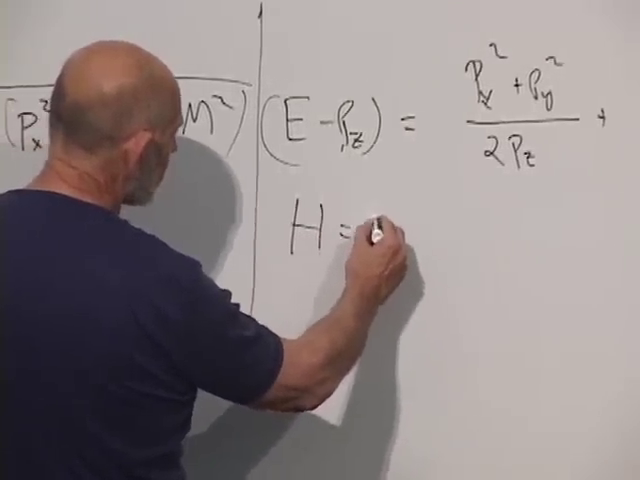
\includegraphics[width=\textwidth]{lecture_02_figure_02.png}
    \par\smallskip\footnotesize (a) Profils à extrémités fixées et de pente nulle.
  \end{minipage}\hfill
  \begin{minipage}[t]{0.48\textwidth}
    \centering
    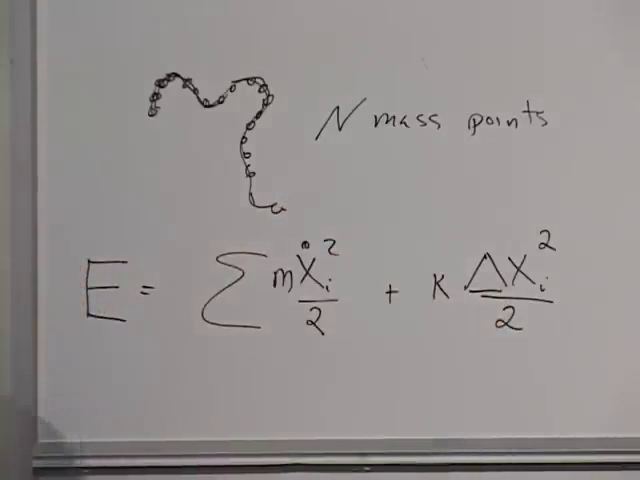
\includegraphics[width=\textwidth]{lecture_02_figure_03.png}
    \par\smallskip\footnotesize (b) Anneaux légers qui coulissent sur des tiges verticales.
  \end{minipage}
  \caption{Les conditions aux limites représentées par des formes et par un dispositif mécanique. Le dispositif des anneaux coulissants donne un sens mécanique sans ambiguïté au mouvement transverse d’une extrémité libre.}
  \lectureframe{00:08:50 and 00:12:15}
  \label{fig:l02-boundaries-board}
\end{figure}

\begin{figure}[H]
  \centering
  \begin{adjustbox}{max width=\linewidth}
  \begin{tikzpicture}[>=Latex,thick,scale=0.92]
    \begin{scope}
      \draw[->] (0,0) -- (4.4,0) node[right] {\(\sigma\)};
      \draw[->] (0,-1.25) -- (0,1.35) node[above] {\(x\)};
      \draw[blue!70!black]
        (0,0) .. controls (0.8,1.1) and (1.4,1.0) .. (2.0,0)
        .. controls (2.7,-1.0) and (3.4,-0.8) .. (4.1,0);
      \fill (0,0) circle (0.06);
      \fill (4.1,0) circle (0.06);
      \node at (2.05,-1.65) {Dirichlet: \(x=0\)};
    \end{scope}
    \begin{scope}[xshift=5.8cm]
      \draw[->] (0,0) -- (4.4,0) node[right] {\(\sigma\)};
      \draw[->] (0,-1.25) -- (0,1.35) node[above] {\(x\)};
      \draw[orange!85!black]
        (0,0.65) .. controls (0.8,0.65) and (1.1,-0.9) .. (2.0,-0.9)
        .. controls (2.9,-0.9) and (3.2,0.55) .. (4.1,0.55);
      \draw[orange!85!black] (0,0.65) -- (0.45,0.65);
      \draw[orange!85!black] (3.65,0.55) -- (4.1,0.55);
      \node at (2.05,-1.65) {Neumann: \(\partial_\sigma x=0\)};
    \end{scope}
  \end{tikzpicture}
  \end{adjustbox}
  \caption{Pour une condition de Dirichlet, la valeur est fixée ; pour une condition de Neumann, c’est la pente qui l’est.}
  \label{fig:l02-boundaries-redraw}
\end{figure}

\begin{classroomqa}
\audiencequestion{Un tuyau d’orgue ouvert ou fermé fournit-il un exemple simple de l’une de ces conditions aux limites ?\lecturetimestamp{00:09:19}}
\lecturerresponse{C’est possible, mais il faut d’abord préciser quelle variable acoustique est développée. La perturbation de pression et le déplacement longitudinal satisfont des conditions idéalisées complémentaires à une extrémité ouverte. Plutôt que de trancher cette question secondaire au tableau, utilisons le modèle des anneaux coulissants : des anneaux presque sans masse peuvent se déplacer verticalement sur les tiges, de sorte que les extrémités de la corde sont libres et que le cas de Neumann s’interprète directement.}
\end{classroomqa}

\begin{classroomqa}
\audiencequestion{Le graphe peut-il avoir une tangente verticale et présenter un saut brutal ?\lecturetimestamp{00:09:53}}
\lecturerresponse{L’analyse de Fourier admet des sauts isolés dans une fonction par morceaux continue. Une corde physique impose des contraintes plus fortes. Un saut disjoint deux points voisins et rend la dérivée spatiale \(\partial_\sigma x\) singulière dans l’énergie continue que nous établirons plus loin. Nous nous limitons donc aux profils continus et dérivables.}
\end{classroomqa}

\begin{classroomqa}
\audiencequestion{Pourquoi l’extrémité ouverte d’un tuyau, ou toute extrémité libre, doit-elle satisfaire une condition aux limites ?\lecturetimestamp{00:11:14}}
\lecturerresponse{L’exemple acoustique dépend du champ choisi et la discussion n’a pas tranché la question. L’exemple mécanique, lui, ne laisse pas d’ambiguïté. Un anneau très léger peut coulisser librement, tout en restant attaché au dernier segment de corde. Nous allons déduire sa condition à partir de la loi de Newton plutôt que de la postuler : une accélération finie à l’extrémité impose que la pente s’annule.}
\end{classroomqa}

\subsection{Les bases de Fourier}

Une fois fixée la classe de conditions aux extrémités, la base de Fourier correspondante est déterminée. Sur \(0\leq\sigma\leq\pi\),

\begin{align}
  x_D(\sigma)
  &=
  \sum_{n=1}^{\infty}x_n\sin(n\sigma),
  \label{eq:l02-dirichlet-series}\\
  x_N(\sigma)
  &=
  \sum_{n=0}^{\infty}x_n\cos(n\sigma).
  \label{eq:l02-neumann-series}
\end{align}

Tous les sinus de \eqref{eq:l02-dirichlet-series} s’annulent aux deux extrémités. Toutes les fonctions cosinus de \eqref{eq:l02-neumann-series} ont une dérivée nulle aux extrémités. Les bornes inférieures diffèrent pour une raison : \(\sin(0\sigma)=0\) ne contribue pas, tandis que \(\cos(0\sigma)=1\) est le mode constant, ou nul. Il représente la valeur moyenne d’une fonction de Neumann.

\begin{figure}[H]
  \centering
  \begin{minipage}[t]{0.48\textwidth}
    \centering
    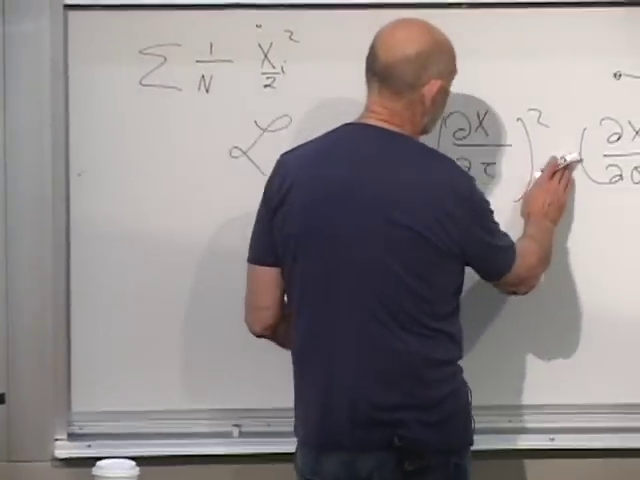
\includegraphics[width=\textwidth]{lecture_02_figure_04.png}
    \par\smallskip\footnotesize (a) Développements en sinus et en cosinus.
  \end{minipage}\hfill
  \begin{minipage}[t]{0.48\textwidth}
    \centering
    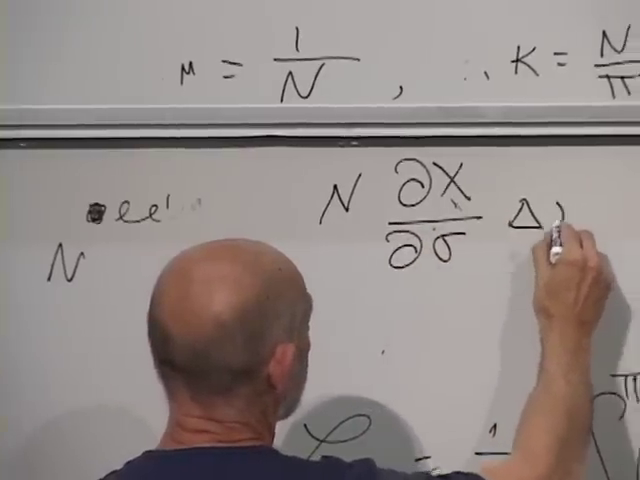
\includegraphics[width=\textwidth]{lecture_02_figure_05.png}
    \par\smallskip\footnotesize (b) Orthogonalité et mode constant exceptionnel.
  \end{minipage}
  \caption{Propriétés de Fourier utilisées plus loin pour diagonaliser la corde.}
  \lectureframe{00:16:15 and 00:20:30}
  \label{fig:l02-fourier-board}
\end{figure}

La dérivation échange les deux classes :

\begin{equation}
  \begin{aligned}
    \partial_\sigma\sin(n\sigma)&=n\cos(n\sigma),\\
    \partial_\sigma\cos(n\sigma)&=-n\sin(n\sigma).
  \end{aligned}
  \label{eq:l02-basis-derivatives}
\end{equation}

Ainsi, la dérivée d’une série de Dirichlet a un comportement de Neumann, et celle d’une série de Neumann a un comportement de Dirichlet. L’orthogonalité élimine alors les termes croisés entre modes distincts :

\begin{align}
  \int_0^\pi\cos(n\sigma)\cos(m\sigma)\,d\sigma
  &=
  \frac{\pi}{2}\delta_{nm},
  && n,m\geq1,
  \label{eq:l02-cos-orthogonality}\\
  \int_0^\pi\sin(n\sigma)\sin(m\sigma)\,d\sigma
  &=
  \frac{\pi}{2}\delta_{nm},
  && n,m\geq1,
  \label{eq:l02-sin-orthogonality}\\
  \int_0^\pi 1\,d\sigma&=\pi .
  \label{eq:l02-zero-norm}
\end{align}

La dernière ligne donne la norme exceptionnelle du cosinus \(n=m=0\). Une constante n’est pas normalisée comme un harmonique non nul ; ce facteur deux distinguera le mode du centre de masse de la corde de ses modes internes.

\subsection{Une formule d’oscillateur à retenir}

Après avoir redimensionné une coordonnée de sorte que la masse mécanique vaille un, un oscillateur obéissant à la loi de Hooke a pour énergie

\begin{align}
  E_{\mathrm{osc}}
  &=
  \frac12\dot q^{\,2}
  +\frac12\omega^2q^2,
  \label{eq:l02-oscillator-energy}\\
  L_{\mathrm{osc}}
  &=
  \frac12\dot q^{\,2}
  -\frac12\omega^2q^2.
  \label{eq:l02-oscillator-lagrangian}
\end{align}

\begin{figure}[H]
  \centering
  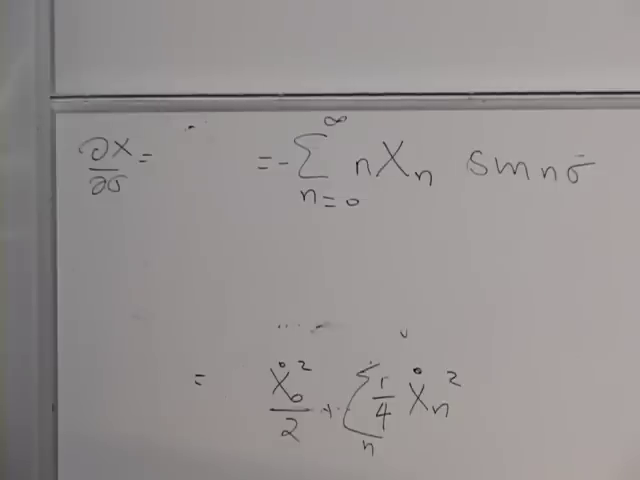
\includegraphics[width=0.68\textwidth]{lecture_02_figure_06.png}
  \caption{L’énergie de l’oscillateur, écrite de façon que le coefficient de \(q^2\) identifie immédiatement \(\omega^2\).}
  \lectureframe{00:24:00}
  \label{fig:l02-oscillator-board}
\end{figure}

Classiquement, \(\omega=\sqrt{\kappa/m}\) ; le redimensionnement de la coordonnée a fixé \(m=1\). En mécanique quantique,

\begin{equation}
  E_Q=\hbar\omega\left(Q+\frac12\right),
  \qquad Q=0,1,2,\ldots .
  \label{eq:l02-oscillator-spectrum}
\end{equation}

Pour les écarts entre niveaux, nous pouvons soustraire le terme commun d’énergie de l’état fondamental et dire que chaque quantum coûte \(\hbar\omega\). Le calcul de la corde procédera d’abord exactement ainsi et remettra à plus tard l’énergie totale du point zéro.

\begin{classroomqa}
\audiencequestion{Comment lit-on la fréquence de l’oscillateur dans la formule de l’énergie ?\lecturetimestamp{00:23:21}}
\lecturerresponse{Avant le redimensionnement, elle vaut \(\omega=\sqrt{\kappa/m}\). Pour une masse unité, le terme de potentiel est \(\frac12\omega^2q^2\) ; son coefficient quadratique est donc le carré de la fréquence.}
\end{classroomqa}

\section{Qu’est-ce qui fait d’un système composite une particule ?}

Une corde est étendue et sera modélisée par de nombreux éléments couplés. En quel sens l’un de ses états quantiques peut-il néanmoins être une particule ? La ponctualité ne peut pas être le critère décisif. Les protons et les neutrons sont composites. Les électrons et les photons sont accompagnés d’un habillage dû aux champs quantiques, bien qu’aucune sous-structure intrinsèque n’ait été mise en évidence. L’image d’un point géométrique classique entouré de rien ne convient pas à une excitation quantique.

La masse et la position du centre de masse ne suffisent pas non plus. Une boîte de gaz possède les deux. Une tasse de café aussi. Pourtant, on n’appelle normalement ni l’une ni l’autre une particule. L’indivisibilité ne convient pas davantage, car un proton est divisible, et le spin ne distingue pas les particules microscopiques des corps macroscopiques.

Le critère utile est l’isolement spectral. Plaçons l’énergie au repos sur un axe vertical et demandons-nous quelle énergie est nécessaire pour atteindre un autre état interne. Juste au-dessus de l’électron, il n’existe pas de série d’excitations électroniques accessible expérimentalement. Le proton, lui, possède des résonances, mais les premières coûtent quelques centaines de MeV, soit une fraction importante de la masse du proton. Ces états sont suffisamment séparés pour être identifiables individuellement.

Une tasse de café, c’est l’inverse. On peut ajouter une énergie arbitrairement petite à un mode sonore de grande longueur d’onde, bousculer une molécule ou produire un phonon. Un nombre immense d’états se pressent dans un intervalle minuscule. À l’échelle du laboratoire, ils forment un continuum. C’est la distinction pratique entre une particule et la \emph{matière informe}.

\begin{figure}[H]
  \centering
  \includegraphics[width=0.58\textwidth]{lecture_02_figure_07.png}
  \caption{Axe vertical de l’énergie au tableau, lors de la comparaison entre le niveau isolé d’une particule et les excitations denses de la matière ordinaire.}
  \lectureframe{00:31:10}
  \label{fig:l02-spectrum-board}
\end{figure}

\begin{figure}[H]
  \centering
  \begin{adjustbox}{max width=\linewidth}
  \begin{tikzpicture}[>=Latex,thick]
    \begin{scope}
      \draw[->] (0,0) -- (0,4.8) node[above] {energy};
      \draw[blue!70!black,line width=1.2pt] (-1.0,0.65) -- (1.0,0.65);
      \draw[blue!70!black,line width=1.2pt] (-1.0,3.65) -- (1.0,3.65);
      \node[right] at (1.05,0.65) {ground state};
      \node[right] at (1.05,3.65) {first internal excitation};
      \draw[<->] (0.65,0.75) -- (0.65,3.55)
        node[midway,right] {large gap};
      \node at (0,-0.55) {particle-like};
    \end{scope}
    \begin{scope}[xshift=7.0cm]
      \draw[->] (0,0) -- (0,4.8) node[above] {energy};
      \foreach \y in {0.55,0.69,0.82,0.94,1.05,1.15,1.24,1.32,1.39,1.45,
        1.51,1.57,1.63,1.70,1.78,1.87,1.97,2.09,2.22,2.36,2.51,2.67,2.84,
        3.02,3.21,3.41,3.62,3.84,4.07}
        \draw[orange!85!black] (-0.95,\y) -- (0.95,\y);
      \node[right] at (1.05,2.25) {dense phonon and internal states};
      \node at (0,-0.55) {macroscopic matter};
    \end{scope}
  \end{tikzpicture}
  \end{adjustbox}
  \caption{Dans ce cours, le critère opérationnel de particule est l’isolement spectral, et non la ponctualité au sens littéral.}
  \label{fig:l02-particle-redraw}
\end{figure}

Ce critère transforme la question philosophique en calcul. Quantifions la corde, déterminons ses niveaux d’énergie internes et examinons leurs espacements. Si le premier état excité de la corde se situe près de l’échelle de Planck tandis que l’état fondamental observé est léger, le gap dépasse de plus de vingt ordres de grandeur les énergies actuelles des accélérateurs. Dans tout le domaine accessible, la corde se comporte alors comme une particule élémentaire.

\begin{classroomqa}
\audiencequestion{Le comportement particulaire dépend-il simplement de l’échelle d’observation ? Si l’on zoome suffisamment, les niveaux cessent-ils d’être distincts ?\lecturetimestamp{00:33:33}}
\lecturerresponse{Un examen à plus petite échelle peut révéler qu’un objet comporte de nombreux constituants, mais il n’efface pas le spectre. La comparaison pertinente porte sur la résolution en énergie de l’expérience et le gap jusqu’à la première excitation interne. Un objet composite peut conserver un comportement particulaire lorsque ce gap est immense.}
\end{classroomqa}

\begin{classroomqa}
\audiencequestion{Pourquoi une corde de violon ordinaire n’est-elle pas une particule ?\lecturetimestamp{00:34:37}}
\lecturerresponse{L’énergie d’un quantum de vibration est incommensurablement petite par rapport à l’énergie au repos de la corde macroscopique. De nombreux états quantiques tiennent donc dans un intervalle relatif minuscule. La corde relève du côté du spectre dense, et non du côté des niveaux isolés.}
\end{classroomqa}

\begin{classroomqa}
\audiencequestion{Les photons et les électrons sont-ils des particules ponctuelles si des fluctuations virtuelles entourent les champs quantiques ?\lecturetimestamp{00:35:40}}
\lecturerresponse{Le mot classique \emph{ponctuel} recouvre trop de choses. L’électron et le photon physiques sont des excitations habillées des champs, mais les expériences n’ont révélé pour aucun des deux de structure intrinsèque en constituants ni de facteur de forme fini. Pour le présent argument, l’essentiel est qu’aucun ne possède une série dense d’états internes presque dégénérés.\editorialnote{Le cours associe le moment magnétique anomal de l’électron à un flou quantique mesurable. Dans la terminologie moderne, ce moment anomal est un effet d’habillage radiatif, et non la preuve d’un rayon fini de l’électron qui aurait été résolu. Par convention, « ponctuel » signifie qu’aucune sous-structure intrinsèque ni aucun facteur de forme n’a été détecté jusqu’à l’échelle sondée.}}
\end{classroomqa}

\begin{classroomqa}
\audiencequestion{La taille d’un photon dépend-elle de sa fréquence ?\lecturetimestamp{00:36:49}}
\lecturerresponse{Sa longueur d’onde, certainement. C’est une notion distincte de la taille intrinsèque de ses constituants. Changer la fréquence modifie le paquet d’ondes et sa longueur d’onde, mais pas un rayon interne du photon qui aurait été résolu.}
\end{classroomqa}

\section{Mécanique transverse exacte à grande impulsion}

Revenons maintenant à la difficulté relativiste. On ne peut pas traiter un bâton en rotation rapide de façon non relativiste en plaçant simplement son centre de masse au repos. Ses extrémités continuent de se déplacer l’une par rapport à l’autre à des vitesses relativistes. C’est le mouvement relatif interne qui rend l’approximation non relativiste invalide.

Il existe cependant une autre limite. Choisissons un axe \(z\) et effectuons une transformation de Lorentz de l’ensemble du système vers une très grande impulsion longitudinale positive \(P_z\). Gardons son impulsion transverse

\begin{equation}
  p_\perp^2=p_x^2+p_y^2
\end{equation}

finie. La projection transverse admet alors une forme hamiltonienne exactement non relativiste dans la limite \(P_z\to\infty\), même si le mouvement interne avant la transformation de Lorentz était relativiste.

\begin{classroomqa}
\audiencequestion{À impulsion infinie, le système massif atteint-il réellement la vitesse de la lumière ?\lecturetimestamp{00:40:43}}
\lecturerresponse{Aucune transformation de Lorentz finie ne l’y amène. On construit des quantités qui ont des limites bien définies lorsque \(P_z\) devient arbitrairement grande. L’expression désigne une procédure limite, et non un état physique à impulsion finie où \(v=c\).}
\end{classroomqa}

\begin{classroomqa}
\audiencequestion{Quel axe faut-il choisir, et qu’en est-il si l’objet tourne autour de cet axe ou dans sa direction transverse ?\lecturetimestamp{00:41:14}}
\lecturerresponse{On peut choisir n’importe quel axe et effectuer la transformation de Lorentz de l’ensemble du système dans cette direction. La mécanique qui reste explicitement en jeu est la projection sur le plan perpendiculaire. Une tige en rotation peut sembler raccourcie ou balayer ce plan, mais sa projection transverse a une forme non relativiste.}
\end{classroomqa}

Les cordes possèdent une propriété supplémentaire qui rend cette représentation particulièrement puissante. En jauge du front de lumière, leurs coordonnées internes longitudinales ne sont pas des oscillateurs indépendants. Les contraintes les déterminent à partir du mouvement transverse. Connaître la corde transverse suffit donc à reconstruire les degrés de liberté physiques.

\begin{classroomqa}
\audiencequestion{L’absence de coordonnée longitudinale indépendante signifie-t-elle que la corde est simplement prise en sandwich dans une couche mince ?\lecturetimestamp{00:42:26}}
\lecturerresponse{La contraction de Lorentz rend effectivement son étendue longitudinale faible dans le référentiel transformé, mais l’affirmation va plus loin. Tout mouvement longitudinal résiduel est contraint par le mouvement transverse ; il ne peut pas être spécifié indépendamment.}
\end{classroomqa}

\begin{classroomqa}
\audiencequestion{Cette réduction aux données transverses est-elle liée au principe holographique ?\lecturetimestamp{00:43:12}}
\lecturerresponse{Elle est étroitement liée au cheminement qui a conduit aux idées holographiques, mais développer ce lien nous éloignerait du calcul présent. Ici, elle justifie simplement de travailler avec la corde transverse.}
\end{classroomqa}

\subsection{Soustraire l’impulsion de la transformation de Lorentz et redimensionner le temps}

Soit \(M\) la masse invariante du système complet, qui inclut les masses des constituants, l’énergie cinétique et l’énergie de liaison. Dans les unités où \(c=1\),

\begin{equation}
  E=\sqrt{P_z^2+p_\perp^2+M^2}.
  \label{eq:l02-relativistic-energy}
\end{equation}

Pour \(P_z\) très grand devant \(p_\perp\) et \(M\),

\begin{equation}
  E
  =
  P_z+\frac{p_\perp^2+M^2}{2P_z}
  +O(P_z^{-3}).
  \label{eq:l02-large-pz}
\end{equation}

\begin{figure}[H]
  \centering
  \includegraphics[width=0.76\textwidth]{lecture_02_figure_08.png}
  \caption{Développement à grande valeur de \(P_z\), avec l’impulsion transverse et la masse invariante conservées.}
  \lectureframe{00:47:30}
  \label{fig:l02-large-pz-board}
\end{figure}

Le terme dominant est grand, mais ne contient aucune information sur l’état interne. Dans un processus qui conserve \(P_z\), comme le passage d’un atome soumis à une transformation de Lorentz entre deux niveaux internes sans changement de son impulsion longitudinale totale, ce terme s’élimine de chaque différence d’énergie. Nous étudions donc

\begin{equation}
  E-P_z=\frac{p_\perp^2+M^2}{2P_z}+O(P_z^{-3}).
  \label{eq:l02-residual-energy}
\end{equation}

Le dénominateur a une signification physique. Comme le hamiltonien engendre l’évolution temporelle, la faible énergie résiduelle indique que l’évolution interne paraît lente dans le temps du laboratoire. C’est la dilatation du temps. Pour conserver le mouvement interne, introduisons un paramètre d’évolution redimensionné \(\tau\), ou, de façon équivalente, multiplions le hamiltonien résiduel par \(P_z\) :

\begin{equation}
  H_\perp
  \equiv
  \lim_{P_z\to\infty}P_z(E-P_z)
  =
  \frac12p_\perp^2+\frac12M^2.
  \label{eq:l02-transverse-hamiltonian}
\end{equation}

\begin{figure}[H]
  \centering
  \begin{minipage}[t]{0.48\textwidth}
    \centering
    \includegraphics[width=\textwidth]{lecture_02_figure_09.png}
    \par\smallskip\footnotesize (a) \(H=i\partial_t\) et le ralentissement de l’évolution interne.
  \end{minipage}\hfill
  \begin{minipage}[t]{0.48\textwidth}
    \centering
    \includegraphics[width=\textwidth]{lecture_02_figure_10.png}
    \par\smallskip\footnotesize (b) Le hamiltonien transverse fini après redimensionnement du temps.
  \end{minipage}
  \caption{De l’énergie résiduelle dilatée dans le temps à un hamiltonien bidimensionnel fini.}
  \lectureframe{00:49:20 and 00:52:40}
  \label{fig:l02-lightfront-board}
\end{figure}

C’est exactement la forme de l’énergie d’une particule de masse unité se déplaçant en deux dimensions : énergie cinétique \(p_\perp^2/2\) plus énergie interne \(M^2/2\). La particularité tient au carré. Dans cette description, la quantité qui joue le rôle de l’énergie au repos ou de liaison est proportionnelle au carré de la masse invariante.\editorialnote{Avec les variables usuelles du front de lumière \(P^\pm=(E\pm P_z)/\sqrt2\), la relation exacte de couche de masse est \(2P^+P^-=p_\perp^2+M^2\). L’équation \eqref{eq:l02-transverse-hamiltonian} correspond à la normalisation à grande valeur de \(P_z\), utilisée dans le cours, de cette même relation invariante.}

\begin{classroomqa}
\audiencequestion{Qu’advient-il des impulsions longitudinales des différentes parties d’un système composite ?\lecturetimestamp{00:51:30}}
\lecturerresponse{Pour un objet composite générique, il faut conserver les fractions de l’impulsion totale \(P_z\) portées par ses constituants. La formule ci-dessus fait intervenir l’impulsion totale du centre de masse. La théorie des cordes est particulière : ses contraintes déterminent le mouvement longitudinal relatif à partir des degrés de liberté transverses, si bien qu’il n’est pas nécessaire d’ajouter un oscillateur longitudinal indépendant.}
\end{classroomqa}

\section{Une corde ouverte discrète}

La corde transformée de Lorentz ne se déplace désormais explicitement que dans le plan transverse. Désignons ses deux coordonnées par \(X\) et \(Y\) et commençons par l’approximer par \(N\) points matériels reliés par \(N-1\) ressorts. Si \(\mu\) est la masse analogue de chaque point et \(k\) la constante de raideur des ressorts entre voisins immédiats, l’énergie vaut

\begin{equation}
  E_N
  =
  \sum_i
  \left[
    \frac{\mu}{2}
    \left(\dot X_i^2+\dot Y_i^2\right)
    +
    \frac{k}{2}
    \left((\Delta X_i)^2+(\Delta Y_i)^2\right)
  \right].
  \label{eq:l02-discrete-energy}
\end{equation}

Chaque terme en \(X\) s’accompagne d’un terme identique en \(Y\), car le plan transverse a deux directions. L’indice \(i\) repère un point le long de la chaîne ; ce n’est pas une coordonnée spatiale.

\begin{figure}[H]
  \centering
  \begin{minipage}[t]{0.48\textwidth}
    \centering
    \includegraphics[width=\textwidth]{lecture_02_figure_11.png}
    \par\smallskip\footnotesize (a) Chaîne de billes et énergie discrète.
  \end{minipage}\hfill
  \begin{minipage}[t]{0.48\textwidth}
    \centering
    \includegraphics[width=\textwidth]{lecture_02_figure_12.png}
    \par\smallskip\footnotesize (b) Comportement à grande valeur de \(N\) pour \(\mu\) et \(k\).
  \end{minipage}
  \caption{La corde ouverte régularisée avant la limite continue.}
  \lectureframe{00:57:42 and 01:02:40}
  \label{fig:l02-chain-board}
\end{figure}

\begin{figure}[H]
  \centering
  \begin{adjustbox}{max width=\linewidth}
  \begin{tikzpicture}[>=Latex,thick]
    \foreach \i in {0,...,8} {
      \coordinate (p\i) at ({1.05*\i},{0.30*sin(55*\i)});
      \filldraw[white] (p\i) circle (0.10);
      \draw (p\i) circle (0.10);
    }
    \foreach \i in {0,...,7} {
      \pgfmathtruncatemacro{\j}{\i+1}
      \draw[decorate,decoration={zigzag,segment length=4pt,amplitude=2pt}]
        (p\i) -- (p\j);
    }
    \node[above=0.35cm of p0] {\(i=0\)};
    \node[above=0.35cm of p8] {\(i=N-1\)};
    \draw[<->] (0,-1.15) -- (8.4,-1.15)
      node[midway,below] {\(0\leq\sigma\leq\pi\)};
    \node at (4.2,1.25)
      {\(\mu=1/N,\quad k=N/\pi^2,\quad\Delta\sigma=\pi/N\)};
  \end{tikzpicture}
  \end{adjustbox}
  \caption{Une image claire de la régularisation. À mesure que la chaîne est affinée, les points s’allègent et les ressorts microscopiques se raidissent.}
  \label{fig:l02-chain-redraw}
\end{figure}

Le paramètre \(\sigma\) repère la position le long de la chaîne. Choisir \(0\leq\sigma\leq\pi\) relève d’une convention, et non d’une mesure de longueur physique. Cela nous rappelle que la corde a deux extrémités. Plus tard, une corde fermée sera paramétrée périodiquement sur \(0\leq\sigma<2\pi\).

La limite continue doit conserver une mécanique collective finie. Une masse fixe pour chaque bille ferait diverger la masse analogue totale ; choisissons donc

\begin{equation}
  \mu=\frac{1}{N}.
  \label{eq:l02-mu-scaling}
\end{equation}

Alors \(N\mu=1\). Il ne s’agit pas de la masse au repos relativiste \(M\), mais du coefficient d’inertie dans le modèle transverse analogue.

Des ressorts montés en série s’assouplissent lorsque leur nombre augmente. Pour conserver une raideur finie à l’échelle de toute la chaîne, chaque ressort microscopique doit donc se raidir :

\begin{equation}
  k=\frac{N}{\pi^2}
  =\frac{1}{\pi\,\Delta\sigma}.
  \label{eq:l02-k-scaling}
\end{equation}

Seule \(k\propto N\) est essentielle. Le facteur \(\pi^2\) est une normalisation choisie pour éliminer les facteurs \(\pi\) indésirables dans les formules continues.

\begin{classroomqa}
\audiencequestion{\(\mu\) est-elle la masse au repos physique de chaque point de la corde ?\lecturetimestamp{01:10:34}}
\lecturerresponse{Non. C’est la masse analogue non relativiste qui intervient dans la chaîne transverse. L’appeler \(M\) risquerait de la confondre avec la masse au repos invariante de l’état relativiste complet de la corde. Pour l’instant, elle sert uniquement à obtenir l’inertie continue correcte.}
\end{classroomqa}

\section{Le système d’ondes continu}

Appliquons les règles établies au début. Puisque \(1/N=\Delta\sigma/\pi\),

\begin{align}
  \sum_i\frac{\mu}{2}\dot X_i^2
  &=
  \frac{1}{2\pi}
  \sum_i\dot X_i^2\,\Delta\sigma
  \longrightarrow
  \frac{1}{2\pi}
  \int_0^\pi
  \left(\partial_\tau X\right)^2d\sigma ,
  \label{eq:l02-kinetic-limit}\\
  \sum_i\frac{k}{2}(\Delta X_i)^2
  &\longrightarrow
  \frac{1}{2\pi}
  \int_0^\pi
  \left(\partial_\sigma X\right)^2d\sigma .
  \label{eq:l02-potential-limit}
\end{align}

Pour la deuxième ligne, utilisons \(\Delta X_i=\partial_\sigma X\,\Delta\sigma\) ainsi que \(k=1/(\pi\Delta\sigma)\). Le même calcul s’applique à \(Y\).

\begin{figure}[H]
  \centering
  \begin{minipage}[t]{0.48\textwidth}
    \centering
    \includegraphics[width=\textwidth]{lecture_02_figure_13.png}
    \par\smallskip\footnotesize (a) Passage de la somme à l’intégrale et de la différence à la dérivée.
  \end{minipage}\hfill
  \begin{minipage}[t]{0.48\textwidth}
    \centering
    \includegraphics[width=\textwidth]{lecture_02_figure_14.png}
    \par\smallskip\footnotesize (b) Énergie continue obtenue.
  \end{minipage}
  \caption{La chaîne discrète devient un champ sur l’intervalle \(\sigma\).}
  \lectureframe{01:05:40 and 01:07:00}
  \label{fig:l02-continuum-board}
\end{figure}

L’énergie et le lagrangien obtenus sont

\begin{align}
  E
  &=
  \frac{1}{2\pi}
  \int_0^\pi d\sigma\,
  \left[
    (\partial_\tau X)^2+(\partial_\tau Y)^2\right.\notag\\[-0.25em]
  &\hspace{6.5em}\left.
    +(\partial_\sigma X)^2+(\partial_\sigma Y)^2
  \right],
  \label{eq:l02-continuum-energy}\\
  L
  &=
  \frac{1}{2\pi}
  \int_0^\pi d\sigma\,
  \left[
    (\partial_\tau X)^2+(\partial_\tau Y)^2\right.\notag\\[-0.25em]
  &\hspace{6.5em}\left.
    -(\partial_\sigma X)^2-(\partial_\sigma Y)^2
  \right].
  \label{eq:l02-continuum-lagrangian}
\end{align}

\begin{figure}[H]
  \centering
  \includegraphics[width=0.78\textwidth]{lecture_02_figure_15.png}
  \caption{Le lagrangien continu, dont les termes cinétique et d’étirement ont des signes opposés.}
  \lectureframe{01:08:48}
  \label{fig:l02-lagrangian-board}
\end{figure}

Si nous rebaptisons \(\sigma\) coordonnée spatiale ordinaire et \(X\) champ \(\phi\), nous obtenons l’énergie et le lagrangien d’un champ d’ondes unidimensionnel. La variation de \eqref{eq:l02-continuum-lagrangian} donne

\begin{equation}
  \left(\partial_\tau^2-\partial_\sigma^2\right)X=0,
  \qquad
  \left(\partial_\tau^2-\partial_\sigma^2\right)Y=0.
  \label{eq:l02-wave-equation}
\end{equation}

Rien dans l’argument immédiat ne nous oblige à résoudre directement ces équations. Il suffit de se représenter des ondes qui se propagent vers la gauche et vers la droite le long de la corde et se réfléchissent à ses extrémités. Une réflexion de Dirichlet inverse le signe du déplacement ; une réflexion de Neumann le conserve.

\begin{classroomqa}
\audiencequestion{Que représente exactement la variable temporelle \(\tau\)\lecturetimestamp{01:08:54}}
\lecturerresponse{C’est le temps redimensionné utilisé pour suivre le mouvement interne dans la description à grande valeur de \(P_z\). Une horloge entraînée avec le système avance lentement par rapport au temps du laboratoire ; \(\tau\) élimine cette dilatation afin que les oscillations internes conservent une fréquence finie. Pour cette mécanique transverse, on peut simplement le traiter comme le temps.\editorialnote{Le cours appelle informellement \(\tau\) le temps propre. Pour une corde étendue, le paramètre d’évolution précis du front de lumière est un temps redimensionné après fixation de jauge, et non un temps propre invariant unique partagé par tous les points. Cela ne change rien à l’argument visé sur la dilatation du temps.}}
\end{classroomqa}

Lorsque le centre de masse est au repos dans le plan transverse, la partie interne de \eqref{eq:l02-continuum-energy} est, dans la normalisation de \eqref{eq:l02-transverse-hamiltonian}, proportionnelle à \(M^2\). C’est pourquoi la quantification de ce système d’ondes apparemment ordinaire révélera le spectre de masse relativiste.

\begin{classroomqa}
\audiencequestion{\(P_z(E-P_z)\) porte-t-il un nom ?\lecturetimestamp{01:11:00}}
\lecturerresponse{On l’appelle couramment énergie du cône de lumière ou du front de lumière. « Front de lumière » décrit mieux l’hypersurface de genre lumière utilisée comme surface d’évolution ; la terminologie traditionnelle n’a pas d’importance pour le calcul.}
\end{classroomqa}

\begin{classroomqa}
\audiencequestion{Le mot « cône » désigne-t-il le cône de lumière usuel de l’espace-temps, et Dirac a-t-il introduit cette terminologie ?\lecturetimestamp{01:11:17}}
\lecturerresponse{La construction en coordonnées nulles peut se représenter avec des axes à 45 degrés, mais la surface d’évolution considérée ici est un front de lumière, et non le cône complet en expansion. Dirac a développé des formulations apparentées de la dynamique relativiste ; la question de l’origine historique du terme est restée ouverte et n’influe pas sur les équations.}
\end{classroomqa}

\section{Pourquoi une extrémité libre satisfait la condition de Neumann}

Nous pouvons maintenant déduire la condition aux extrémités au lieu de la postuler. La loi de Newton s’applique, car la mécanique transverse après la transformation de Lorentz a exactement la forme non relativiste. Un point matériel intérieur est tiré par des ressorts des deux côtés. Le point à l’extrémité ne subit la traction que du ressort qui le relie à son voisin.

\begin{classroomqa}
\audiencequestion{Pourquoi pouvons-nous utiliser la loi de Newton tout en étudiant une corde relativiste ?\lecturetimestamp{01:14:52}}
\lecturerresponse{Nous n’appliquons pas la mécanique newtonienne au mouvement complet dans l’espace-temps avant la transformation de Lorentz. Nous l’appliquons aux variables transverses de la description à impulsion infinie, dont le hamiltonien a exactement la forme non relativiste.}
\end{classroomqa}

À l’extrémité droite, la loi de Hooke donne, au signe près selon l’orientation,

\begin{equation}
  F_{\mathrm{end}}
  =
  -k\,\Delta X
  =
  -\frac{1}{\pi\Delta\sigma}
   \left(\partial_\sigma X\,\Delta\sigma\right)
  =
  -\frac{1}{\pi}\partial_\sigma X .
  \label{eq:l02-endpoint-force}
\end{equation}

\begin{figure}[H]
  \centering
  \begin{minipage}[t]{0.48\textwidth}
    \centering
    \includegraphics[width=\textwidth]{lecture_02_figure_16.png}
    \par\smallskip\footnotesize (a) Force à l’extrémité proportionnelle à la pente locale.
  \end{minipage}\hfill
  \begin{minipage}[t]{0.48\textwidth}
    \centering
    \includegraphics[width=\textwidth]{lecture_02_figure_17.png}
    \par\smallskip\footnotesize (b) Condition d’accélération finie.
  \end{minipage}
  \caption{Déduction de la condition aux limites d’extrémité libre à partir de la loi de Newton.}
  \lectureframe{01:18:20 and 01:20:10}
  \label{fig:l02-neumann-board}
\end{figure}

L’équation de Newton pour le point terminal est

\begin{equation}
  \mu\,\partial_\tau^2X=F_{\mathrm{end}},
  \qquad
  \mu=\frac1N=\frac{\Delta\sigma}{\pi}.
  \label{eq:l02-endpoint-newton}
\end{equation}

En combinant \eqref{eq:l02-endpoint-force} et \eqref{eq:l02-endpoint-newton},

\begin{equation}
  \partial_\sigma X
  =
  -\Delta\sigma\,\partial_\tau^2X
  \quad\text{at the right endpoint},
  \label{eq:l02-endpoint-scaling}
\end{equation}

avec le signe de la force inversé à l’extrémité gauche. Si \(\partial_\sigma X\) tendait vers une constante non nulle tandis que \(\Delta\sigma\to0\), l’accélération de l’extrémité divergerait comme \(N\). Une limite continue raisonnable avec accélération finie exige donc

\begin{equation}
  \left.\partial_\sigma X\right|_{0,\pi}=0,
  \qquad
  \left.\partial_\sigma Y\right|_{0,\pi}=0.
  \label{eq:l02-open-neumann}
\end{equation}

\begin{figure}[H]
  \centering
  \begin{adjustbox}{max width=\linewidth}
  \begin{tikzpicture}[>=Latex,thick,scale=1.0]
    \coordinate (a) at (0,0);
    \coordinate (b) at (4.5,0.75);
    \filldraw[white] (a) circle (0.12);
    \draw (a) circle (0.12);
    \filldraw[white] (b) circle (0.12);
    \draw (b) circle (0.12);
    \draw[decorate,decoration={zigzag,segment length=6pt,amplitude=3pt}]
      (a) -- (b);
    \draw[dashed] (a) -- (0,-1.2);
    \draw[dashed] (b) -- (4.5,-1.2);
    \draw[<->] (4.85,0) -- (4.85,0.75)
      node[midway,right] {\(\Delta X\)};
    \draw[->,red!70!black] (b) -- (5.75,0.95)
      node[right] {\(F_{\rm end}=-k\Delta X\)};
    \node[below] at (0,-1.2) {\(N-1\)};
    \node[below] at (4.5,-1.2) {\(N\)};
    \node at (2.5,-2.0)
      {\(\mu\ddot X=-k\Delta X
      \ \Longrightarrow\
      \partial_\sigma X=-\Delta\sigma\,\ddot X\to0\)};
  \end{tikzpicture}
  \end{adjustbox}
  \caption{Dans la limite de régularisation, la masse du dernier point tend vers zéro. Une accélération finie n’est possible que si la pente à l’extrémité s’annule.}
  \label{fig:l02-neumann-redraw}
\end{figure}

Le même argument aux deux extrémités et dans les deux directions transverses donne des conditions aux limites de Neumann pour une corde ouverte libre.

\section{Modes normaux de la corde ouverte}

Nous disposons maintenant d’un système classique complet : un lagrangien et ses conditions aux limites. Après l’analyse de Fourier, la quantification devient simple. Comme les extrémités sont de Neumann,

\begin{align}
  X(\sigma,\tau)
  &=
  \sum_{n=0}^{\infty}X_n(\tau)\cos(n\sigma),
  \label{eq:l02-X-expansion}\\
  Y(\sigma,\tau)
  &=
  \sum_{n=0}^{\infty}Y_n(\tau)\cos(n\sigma).
  \label{eq:l02-Y-expansion}
\end{align}

Toute la dépendance en \(\sigma\) est portée par les cosinus. Toute la dépendance temporelle est portée par les coefficients ; la corde oscille parce que \(X_n(\tau)\) et \(Y_n(\tau)\) varient.

\begin{figure}[H]
  \centering
  \includegraphics[width=0.78\textwidth]{lecture_02_figure_18.png}
  \caption{Développement en modes de Neumann, placé à côté de la relation d’orthogonalité qui réduira les sommes doubles.}
  \lectureframe{01:21:45}
  \label{fig:l02-mode-expansion-board}
\end{figure}

\subsection{Terme cinétique et mode zéro}

La dérivation par rapport au temps donne

\begin{equation}
  \partial_\tau X
  =
  \sum_{n=0}^{\infty}\dot X_n(\tau)\cos(n\sigma).
  \label{eq:l02-time-mode}
\end{equation}

Le carré produit une somme double sur \(n\) et \(m\), mais
\eqref{eq:l02-cos-orthogonality} annule tous les termes pour lesquels \(n\neq m\).
En traitant séparément le mode constant,

\begin{equation}
  \frac{1}{2\pi}\int_0^\pi
  (\partial_\tau X)^2\,d\sigma
  =
  \frac12\dot X_0^{\,2}
  +
  \frac14\sum_{n=1}^{\infty}\dot X_n^{\,2}.
  \label{eq:l02-mode-kinetic}
\end{equation}

\begin{figure}[H]
  \centering
  \includegraphics[width=0.76\textwidth]{lecture_02_figure_19.png}
  \caption{L’intégrale d’orthogonalité réduit la somme double du terme cinétique au mode zéro et à une somme diagonale.}
  \lectureframe{01:29:10}
  \label{fig:l02-mode-kinetic-board}
\end{figure}

Le coefficient constant est la position moyenne,

\begin{equation}
  X_0(\tau)=\frac1\pi\int_0^\pi X(\sigma,\tau)\,d\sigma ,
  \label{eq:l02-center-of-mass}
\end{equation}

et de même pour \(Y_0\). Avec une densité de masse uniforme analogue, ces coordonnées sont celles du centre de masse. Elles ont une énergie cinétique, mais aucune force de rappel : la corde entière peut se déplacer librement dans le plan transverse.

\subsection{Terme d’étirement et fréquences des oscillateurs}

La dérivation spatiale donne

\begin{equation}
  \partial_\sigma X
  =
  -\sum_{n=1}^{\infty}nX_n(\tau)\sin(n\sigma).
  \label{eq:l02-spatial-mode}
\end{equation}

Le mode zéro disparaît, car une translation uniforme n’étire pas la corde. En utilisant l’orthogonalité des sinus,

\begin{equation}
  \frac{1}{2\pi}\int_0^\pi
  (\partial_\sigma X)^2\,d\sigma
  =
  \frac14\sum_{n=1}^{\infty}n^2X_n^{\,2}.
  \label{eq:l02-mode-potential}
\end{equation}

\begin{figure}[H]
  \centering
  \includegraphics[width=0.76\textwidth]{lecture_02_figure_20.png}
  \caption{La dérivation de la série de cosinus produit la somme double de sinus ; l’orthogonalité impose de nouveau \(n=m\).}
  \lectureframe{01:31:40}
  \label{fig:l02-mode-potential-board}
\end{figure}

Le lagrangien du secteur \(X\) s’écrit donc

\begin{equation}
  L_X
  =
  \frac12\dot X_0^{\,2}
  +
  \frac14\sum_{n=1}^{\infty}
  \left(
    \dot X_n^{\,2}-n^2X_n^{\,2}
  \right),
  \label{eq:l02-X-lagrangian}
\end{equation}

avec une expression identique pour \(Y\). L’énergie correspondante comporte un signe plus devant \(n^2X_n^2\). Chaque mode non nul est un oscillateur harmonique indépendant et, par comparaison avec \eqref{eq:l02-oscillator-lagrangian}, on obtient

\begin{equation}
  \omega_n=n,
  \qquad n=1,2,3,\ldots .
  \label{eq:l02-mode-frequency}
\end{equation}

\begin{figure}[H]
  \centering
  \includegraphics[width=0.80\textwidth]{lecture_02_figure_21.png}
  \caption{Le lagrangien des oscillateurs découplés et la conclusion \(\omega_n=n\), avec la tour identique de \(Y\) indiquée ci-dessous.}
  \lectureframe{01:35:50}
  \label{fig:l02-oscillator-modes-board}
\end{figure}

Les modes normaux sont simplement les harmoniques de la corde. Le premier se courbe lentement, le deuxième a une fréquence deux fois plus élevée, le troisième trois fois plus élevée, et ainsi de suite. Dans la théorie libre, l’orthogonalité empêche tout couplage entre harmoniques.

\begin{classroomqa}
\audiencequestion{Que devient l’oscillateur \(n=0\) ?\lecturetimestamp{01:34:49}}
\lecturerresponse{Sa fréquence est nulle, car il ne s’agit pas du tout d’un oscillateur interne. Il traduit le centre de masse. Aucun ressort ne ramène la corde entière à une position transverse privilégiée : le mode zéro est donc une coordonnée de particule libre.}
\end{classroomqa}

En supprimant le terme cinétique du centre de masse, il reste l’énergie interne

\begin{equation}
  E_{\mathrm{int}}
  =
  \frac14
  \sum_{n=1}^{\infty}
  \left[
    \dot X_n^{\,2}+n^2X_n^{\,2}
    +\dot Y_n^{\,2}+n^2Y_n^{\,2}
  \right].
  \label{eq:l02-internal-energy}
\end{equation}

Dans la normalisation du cône de lumière, cette énergie est proportionnelle au carré de la masse invariante de l’état de la corde. Nous avons ainsi ramené le problème relativiste de la masse à la mécanique quantique de deux tours dénombrables d’oscillateurs.

\section{Niveaux quantifiés et comportement particulaire}

Soit \(a_n^\dagger\) l’opérateur qui crée un quantum dans l’oscillateur \(X\) de fréquence
\(n\), et \(b_n^\dagger\) celui qui fait de même pour \(Y\). Le cours remet à plus tard le traitement systématique des opérateurs, mais cette notation rend le dénombrement des niveaux transparent. Par rapport au décalage de l’état fondamental,

\begin{equation}
  \begin{aligned}
    \Delta E_{\mathrm{int}}
    &=\sum_{n=1}^{\infty}n\left(Q_n^X+Q_n^Y\right),\\
    Q_n^X,Q_n^Y&\in\{0,1,2,\ldots\}.
  \end{aligned}
  \label{eq:l02-quantized-energy}
\end{equation}

où \(\hbar=1\). L’entier \(n\) indique quel oscillateur est excité ;
\(Q_n\) compte le nombre de quanta qu’il contient.\editorialnote{Chaque oscillateur contribue aussi une énergie de point zéro. La somme
infinie nécessite une régularisation et fournit l’intercept de la formule de masse de la corde. Le cours laisse délibérément indéterminé ici le décalage de l’état fondamental et ne dénombre que les niveaux d’excitation.}

Le vide des oscillateurs \(\ket{0}\) n’est pas le vide de l’espace-temps. Il s’agit d’une corde ouverte sans aucun oscillateur interne excité. Elle possède une énergie, une quantité de mouvement et une place bien définie dans le spectre de la corde.

Au premier niveau, il y a deux états,

\begin{equation}
  a_1^\dagger\ket{0},
  \qquad
  b_1^\dagger\ket{0},
  \label{eq:l02-level-one}
\end{equation}

qui correspondent au premier harmonique, polarisé selon \(X\) ou \(Y\).
Des combinaisons linéaires décrivent toute polarisation transverse.

Au deuxième niveau, il y a cinq états :

\begin{equation}
  (a_1^\dagger)^2\ket{0},
  \quad
  a_1^\dagger b_1^\dagger\ket{0},
  \quad
  (b_1^\dagger)^2\ket{0},
  \quad
  a_2^\dagger\ket{0},
  \quad
  b_2^\dagger\ket{0}.
  \label{eq:l02-level-two}
\end{equation}

Trois utilisent deux quanta du premier harmonique ; deux utilisent un quantum du deuxième harmonique. Les deux constructions coûtent deux unités.

\begin{figure}[H]
  \centering
  \includegraphics[width=0.76\textwidth]{lecture_02_figure_22.png}
  \caption{Les cinq états du deuxième niveau, dénombrés de nouveau après une question de l’auditoire : deux excitations doubles, une excitation mixte et deux excitations du deuxième harmonique.}
  \lectureframe{01:44:00}
  \label{fig:l02-levels-board}
\end{figure}

\begin{figure}[H]
  \centering
  \begin{adjustbox}{max width=\linewidth}
  \begin{tikzpicture}[>=Latex,thick]
    \draw[->] (0,0) -- (0,5.1) node[above] {\(\Delta E_{\rm int}\)};
    \draw[blue!70!black] (-0.65,0.55) -- (0.65,0.55);
    \node[right] at (0.85,0.55) {\(\ket{0}\) \quad multiplicity \(1\)};
    \draw[blue!70!black] (-0.65,2.15) -- (0.65,2.15);
    \node[right] at (0.85,2.15)
      {\(a_1^\dagger\ket{0},\ b_1^\dagger\ket{0}\)
      \quad multiplicity \(2\)};
    \draw[blue!70!black] (-0.65,3.75) -- (0.65,3.75);
    \node[right,text width=8.6cm] at (0.85,3.75)
      {\((a_1^\dagger)^2\ket{0},
      a_1^\dagger b_1^\dagger\ket{0},
      (b_1^\dagger)^2\ket{0},
      a_2^\dagger\ket{0},\ b_2^\dagger\ket{0}\)
      \quad multiplicity \(5\)};
    \node[left] at (-0.75,0.55) {\(0\)};
    \node[left] at (-0.75,2.15) {\(1\)};
    \node[left] at (-0.75,3.75) {\(2\)};
  \end{tikzpicture}
  \end{adjustbox}
  \caption{Les trois premiers niveaux d’excitation de la corde ouverte à deux directions transverses.}
  \label{fig:l02-levels-redraw}
\end{figure}

\begin{classroomqa}
\audiencequestion{Y a-t-il quatre ou cinq états au deuxième niveau excité ?\lecturetimestamp{01:43:04}}
\lecturerresponse{Cinq. Exciter \(X_1\) deux fois, exciter \(Y_1\) deux fois et exciter chacun une fois donnent trois états. En exciter \(X_2\) une fois ou \(Y_2\) une fois en donnent deux de plus. L’exercice proposé consiste à dénombrer les deux niveaux suivants.}
\end{classroomqa}

La conclusion essentielle est déjà visible. Les niveaux successifs sont séparés par des écarts finis, et chacun possède une multiplicité finie. Selon le critère spectral qui la distingue du café, du gaz ou d’une corde de violon ordinaire, la corde quantifiée se comporte donc comme une particule. Nous déterminerons plus tard quels états sont physiquement acceptables et quelles pathologies doivent être éliminées.

\section{Pourquoi les interactions des cordes ouvertes produisent des cordes fermées}

Une corde ouverte a deux extrémités. Ses interactions élémentaires consistent à joindre et à scinder des cordes. Dans le modèle hadronique, on peut imaginer un quark à une extrémité et un antiquark à l’autre ; leur annihilation joint deux segments de corde. Les cordes fondamentales qui nous intéresseront plus tard ne sont pas nécessairement associées à cette interprétation littérale des extrémités hadroniques, mais la règle locale de jonction demeure.

Considérons maintenant une corde ouverte qui fluctue jusqu’à ce que ses deux extrémités se rapprochent. Localement, une extrémité ne peut pas savoir si l’autre appartient à la même corde ou à une corde différente. Si les extrémités peuvent se joindre, elles peuvent le faire ici et produire une boucle fermée.

\begin{figure}[H]
  \centering
  \includegraphics[width=0.70\textwidth]{lecture_02_figure_23.png}
  \caption{Schéma au tableau d’une corde ouverte qui fluctue jusqu’à ce que ses deux extrémités se rejoignent et forment une boucle fermée.}
  \lectureframe{01:47:00}
  \label{fig:l02-closed-board}
\end{figure}

\begin{figure}[H]
  \centering
  \begin{adjustbox}{max width=\linewidth}
  \begin{tikzpicture}[>=Latex,thick]
    \begin{scope}
      \draw[blue!70!black]
        (0,0) .. controls (0.8,1.2) and (1.7,-1.0) .. (2.6,0.45)
        .. controls (3.4,1.55) and (4.0,0.3) .. (4.7,0.85);
      \fill (0,0) circle (0.09);
      \fill (4.7,0.85) circle (0.09);
      \node at (2.35,-1.25) {open string fluctuation};
    \end{scope}
    \draw[->,line width=1pt] (5.25,0.3) -- (6.65,0.3)
      node[midway,above] {join};
    \begin{scope}[xshift=8.1cm]
      \draw[orange!85!black]
        (0,0) .. controls (0.3,1.5) and (2.5,1.8) .. (3.1,0.3)
        .. controls (3.5,-1.1) and (0.7,-1.5) .. (0,0);
      \node at (1.55,-1.85) {closed string};
    \end{scope}
  \end{tikzpicture}
  \end{adjustbox}
  \caption{Dès lors que la jonction des extrémités est possible, une corde ouverte peut se refermer sur elle-même.}
  \label{fig:l02-closed-redraw}
\end{figure}

Une théorie peut donc contenir des cordes fermées sans cordes ouvertes, mais une théorie en interaction qui contient des cordes ouvertes ne peut pas exclure les cordes fermées de façon cohérente. Cette asymétrie est la prédiction importante. Les identifications spectrales seront développées plus tard, mais on en voit déjà l’aboutissement : les états sans masse des cordes ouvertes fournissent souvent des particules de jauge comme les photons, tandis que le spectre des cordes fermées contient un état sans masse de spin deux, le graviton. Dès que la théorie des cordes est en interaction, les cordes fermées, et donc la gravité, ne sont pas un ajout facultatif.
